%!TEX root=../../root.tex

Now, we have all we need to introduce CNNs. On the surface, CNNs are just normal feed-forward neural networks in which in each layer, instead of the linear operation of matrix multiplication with the weights and biases, we have another linear operation: convolution.

\begin{figure}[H]
    \centering
    \begin{overpic}
        [trim=0cm 0cm 0cm 0cm,clip,width=0.95\linewidth]{08/dnn1_.pdf}
    %
            \put(-2.75,30.25){\footnotesize $f_1^\mathrm{in}(x)$}
            \put(-2.75,22.5){\footnotesize $f_2^\mathrm{in}(x)$}
            \put(-2.75,5.5){\footnotesize $f_n^\mathrm{in}(x)$}
    %
            \put(23.5,33){\footnotesize $g_1^{(1)}(x)$}
            \put(23.5,25.25){\footnotesize $g_2^{(1)}(x)$}
            \put(23.5,8.25){\footnotesize $g_{m_1}^{(1)}(x)$}
    %
            \put(44.75,33){\footnotesize $g_1^{(2)}(x)$}
            \put(44.75,25.25){\footnotesize $g_2^{(2)}(x)$}
            \put(44.75,8.25){\footnotesize $g_{m_2}^{(2)}(x)$}
    %
            \put(63.25,33){\footnotesize $g_1^{(3)}(x)$}
            \put(63.25,25.25){\footnotesize $g_2^{(3)}(x)$}
            \put(63.25,8.25){\footnotesize $g_{m_3}^{(3)}(x)$}
    %
            \put(76.5,33){\footnotesize $g_1^{(L-1)}(x)$}
            \put(76.5,25.25){\footnotesize $g_2^{(L-1)}(x)$}
            \put(76.5,8.25){\footnotesize $g_{m_{L-1}}^{(L-1)}(x)$}
            %
            \put(93.5,30.25){\footnotesize $g_1^\mathrm{out}(x)$}
            \put(93.5,22.5){\footnotesize $g_2^\mathrm{out}(x)$}
            \put(93.5,5.5){\footnotesize $g_m^\mathrm{out}(x)$}	
            %
            %
    %
            \put(15,3){\footnotesize $W^{(1)}$}			
            \put(36,3){\footnotesize $W^{(2)}$}	
            \put(57,3){\footnotesize $W^{(3)}$}	
            \put(82,3){\footnotesize $W^{(L)}$}					
        \end{overpic}
    \caption{CNN consisting of $L$ convolutional layers. Notice the architecture superficially is identical to a feed-forward neural network.}
\end{figure}

This modified version of the network layer (unsurprisingly) takes the name of \emph{convolutional layer}. Such layers perform the following operation on the incoming data:
\begin{equation}
    g^{(k)}_\ell(x) = \sigma\left( \displaystyle\sum_{\ell'=1}^{m_{k-1}} (g^{(k-1)}_{\ell'} \star w^{(k)}_{\ell,\ell'}) (x) \right) \hspace{1.5mm} 
    \begin{array}{l}
    \ell = 1, \hdots, m_k\\
     \ell' = 1, \hdots, m_{k-1}\\
    \end{array}
\end{equation}
in which the activation function is left unchanged, but the parameters are no longer weight matrices but \textit{filter} (or \textit{kernel}) matrices. If the data under consideration are images, then the incoming $g^{(k-1)}_{\ell'}$ are feature maps computed by the earlier convolutional layer, that still have the shape of images (although maybe with different dimensions), and thus that can be again convoluted in the current layer.

Where is the advantage? Well for starters, we have seen how the convolutional operator by itself implements shift-equivariance, one of our desirable priors. Then, we have a huge gain in computational complexity, since the number of parameters per filter is \emph{constant} with respect to the size of the input, while instead in the standard MLP a fully-connected layer has a weight matrix that must have dimensions matching the incoming and outcoming shape of the data. 

This is possible since the \textit{same filter} is applied to the whole data (across the whole image), and hence we have \emph{weight sharing}. In fact, if we apply \cref{eq:08:03:conv-sum} with the first term being the earlier feature map and the second being the filter, we have
\begin{equation}
    (g^{(k-1)}_{\ell'} \star w^{(k)}_{\ell,\ell'}) (x) [m, n] = \sum_i\sum_j  g^{(k-1)}_{\ell'} [i,j] \, w^{(k)}_{\ell,\ell'}[m-i,n-j].
\end{equation}
in which $i, j$ will span the filter (according to the boundary condition), eventually spanning all its weights, therefore the same weights will be used also to compute the other locations of the current feature map.

This fact leads to weight sharing and efficient computation (since the complexity of the sums above depend on the size of the filters, that do not depend on the size of the input), but also to \emph{sparse interactions}. In fact, not every location of the earlier feature map will be used to compute a single location of the current feature map, but only the ones ``covered'' by the filter.

\begin{figure}[H]
    \centering
    \begin{subfigure}[t]{0.45\textwidth}
        \centering
        \begin{overpic}[width=\linewidth]{08/fcn}\end{overpic}
        \caption{Fully-connected layer: The outgoing edges from the input node $x_3$ have different weights than the ones outgoing from the other nodes.}
    \end{subfigure}
    \hfill
    \begin{subfigure}[t]{0.45\textwidth}
        \centering
        \begin{overpic}[width=\linewidth]{08/convlayer}\end{overpic}
        \caption{Convolutional layer: The outgoing edges from the input node $x_3$ have \emph{the same} weights of the ones outgoing from the other nodes. Furthermore, notice that there are fewer edges in general, leading to \emph{sparse interactions}.}
    \end{subfigure}
    \caption{Visualization of weight sharing.}
\end{figure}



This is not all however. The other main architectural difference is the introduction of another new operation: \emph{pooling}. A pooling function replaces the output of the net at a certain location with a summary statistic of the nearby outputs (its \textit{neighborhood}). The most used pooling functions are the \emph{max pooling} that replaces the neighborhood with its maximum value and the \emph{avg pooling} that instead does so with its average value.

\begin{figure}[H]
    \centering
    \begin{overpic}
        [width=1\linewidth]{08/maxpool1}
        \put(7,-2){\small Input data}
        \put(36,5){\small Filter}
        \put(59,-2){\small Feature map}
        %
        \put(84,11){\small Max pooling}
    \end{overpic}
    \caption{Pooling operation.}
\end{figure}

\begin{figure}[H]
    \centering
    \begin{overpic}
        [trim=0cm 0cm 0cm 0cm,clip,width=0.95\linewidth]{08/dnn2_.pdf}
            \put(-2.75,30.25){\footnotesize $f_1^\mathrm{in}(x)$}
            \put(-2.75,22.5){\footnotesize $f_2^\mathrm{in}(x)$}
            \put(-2.75,5.5){\footnotesize $f_n^\mathrm{in}(x)$}

            \put(93.5,30.25){\footnotesize $g_1^\mathrm{out}(x)$}
            \put(93.5,22.5){\footnotesize $g_2^\mathrm{out}(x)$}
            \put(93.5,5.5){\footnotesize $g_m^\mathrm{out}(x)$}	

            \put(15,3){\footnotesize $W^{(1)}$}			
            \put(39,3){\footnotesize $W^{(2)}$}	
            \put(60,3){\footnotesize $W^{(3)}$}	
            \put(81,3){\footnotesize $W^{(L)}$}						
    \end{overpic}
    \caption{CNN consisting of $L$ convolutional layers interleaved with pooling}
\end{figure}

The use of pooling can be viewed as adding an infinitely strong prior that
the function the layer learns must be invariant to small translations. This allows to capture non-local interactions via simple building blocks that only describe sparse interactions. Furthermore, if we pool over the outputs of separately parametrized convolutions (different layers), the features can learn which transformations to become invariant to. 

Pooling also serves as a \emph{subsampling} operator, reducing the size of the data and thus the computational and statistical burden on the next layer.

\begin{figure}[H]
    \begin{center}
    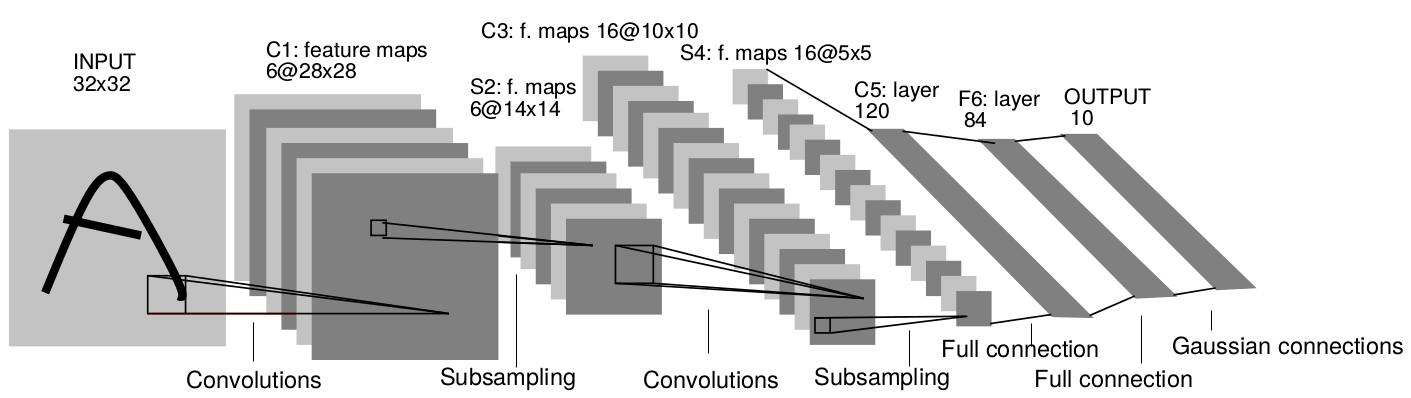
\includegraphics[width=\textwidth]{08/cnn.png}
    \end{center}
    \caption{Convolution and downsampling (pooling) operations give the typical shape of a CNN, with data decreasing in size but filters increasing in number, then followed by fully-connected layers to perform other tasks like classification, based on the representation of the data the previous layers have extracted.}
\end{figure}

\begin{figure}[H]
    \centering
    \begin{overpic}
        [trim=0cm 0cm 0cm 0cm,clip,width=0.8\linewidth]{08/car}
        \put(20,49){$\to$}
        \put(25,51){\footnotesize low-level}
        \put(25.5,48){\footnotesize features}
        \put(38,49){$\to$}
        \put(43,51){\footnotesize mid-level}
        \put(43.5,48){\footnotesize features}
        \put(57,49){$\to$}
        \put(62.5,51){\footnotesize hi-level}
        \put(62,48){\footnotesize features}
        \put(74,49){$\to$}
        \put(78,49){ ``car''}
    \end{overpic}
    \caption{Empirically it has been shown that it is possible to interpret the CNN architecture as learning increasingly more complex features.}
\end{figure}
